%%%%%%%%%%%%%%%%%%%%%%%%%%%%%%%%%%%%%%%%%
% Journal Article
% LaTeX Template
% Version 1.4 (15/5/16)
%
% This template has been downloaded from:
% http://www.LaTeXTemplates.com
%
% Original author:
% Frits Wenneker (http://www.howtotex.com) with extensive modifications by
% Vel (vel@LaTeXTemplates.com)
%
% License:
% CC BY-NC-SA 3.0 (http://creativecommons.org/licenses/by-nc-sa/3.0/)
%
%%%%%%%%%%%%%%%%%%%%%%%%%%%%%%%%%%%%%%%%%

%----------------------------------------------------------------------------------------
%	PACKAGES AND OTHER DOCUMENT CONFIGURATIONS
%----------------------------------------------------------------------------------------

\documentclass[twoside,twocolumn]{article}

\usepackage{blindtext} % Package to generate dummy text throughout this template 

\usepackage[sc]{mathpazo} % Use the Palatino font
\usepackage[T1]{fontenc} % Use 8-bit encoding that has 256 glyphs
\linespread{1.05} % Line spacing - Palatino needs more space between lines
\usepackage{microtype} % Slightly tweak font spacing for aesthetics

\usepackage[english]{babel} % Language hyphenation and typographical rules

\usepackage[hmarginratio=1:1,top=32mm,columnsep=20pt]{geometry} % Document margins
\usepackage[hang, small,labelfont=bf,up,textfont=it,up]{caption} % Custom captions under/above floats in tables or figures
\usepackage{booktabs} % Horizontal rules in tables

\usepackage{lettrine} % The lettrine is the first enlarged letter at the beginning of the text

\usepackage{enumitem} % Customized lists
\setlist[itemize]{noitemsep} % Make itemize lists more compact

\usepackage{abstract} % Allows abstract customization
\renewcommand{\abstractnamefont}{\normalfont\bfseries} % Set the "Abstract" text to bold
\renewcommand{\abstracttextfont}{\normalfont\small\itshape} % Set the abstract itself to small italic text

\usepackage{titlesec} % Allows customization of titles
\renewcommand\thesection{\Roman{section}} % Roman numerals for the sections
\renewcommand\thesubsection{\roman{subsection}} % roman numerals for subsections
\titleformat{\section}[block]{\large\scshape\centering}{\thesection.}{1em}{} % Change the look of the section titles
\titleformat{\subsection}[block]{\large}{\thesubsection.}{1em}{} % Change the look of the section titles

\usepackage{fancyhdr} % Headers and footers
\pagestyle{fancy} % All pages have headers and footers
\fancyhead{} % Blank out the default header
\fancyfoot{} % Blank out the default footer
\fancyhead[C]{Running title $\bullet$ May 2016 $\bullet$ Vol. XXI, No. 1} % Custom header text
\fancyfoot[RO,LE]{\thepage} % Custom footer text

\usepackage{titling} % Customizing the title section

\usepackage{hyperref} % For hyperlinks in the PDF

%----------------------------------------------------------------------------------------
%	TITLE SECTION
%----------------------------------------------------------------------------------------

\setlength{\droptitle}{-4\baselineskip} % Move the title up

\pretitle{\begin{center}\Huge\bfseries} % Article title formatting
\posttitle{\end{center}} % Article title closing formatting
\title{Article Title} % Article title
\author{%
\textsc{John Smith}\thanks{A thank you or further information} \\[1ex] % Your name
\normalsize University of California \\ % Your institution
\normalsize \href{mailto:john@smith.com}{john@smith.com} % Your email address
%\and % Uncomment if 2 authors are required, duplicate these 4 lines if more
%\textsc{Jane Smith}\thanks{Corresponding author} \\[1ex] % Second author's name
%\normalsize University of Utah \\ % Second author's institution
%\normalsize \href{mailto:jane@smith.com}{jane@smith.com} % Second author's email address
}
\date{\today} % Leave empty to omit a date
\renewcommand{\maketitlehookd}{%
\begin{abstract}
\noindent \blindtext % Dummy abstract text - replace \blindtext with your abstract text
\end{abstract}
}

%----------------------------------------------------------------------------------------

\begin{document}

% Print the title
\maketitle

%----------------------------------------------------------------------------------------
%	ARTICLE CONTENTS
%----------------------------------------------------------------------------------------

\section{Introduction}

% Need for autonomous sytems
% Need for systems to support user
% Requirements: alignment of objectives and system transparency

\lettrine[nindent=0em,lines=3]{U}nmanned vehicles are becoming an essential part of the battlefield (Chen et al, 2011). However, currents UVs are mostly controlled remotely by a single or more operators, so the increasing use of UVs requires even more man power to control these systems. This increases the operating and training cost and it challenges the demand for more UV operations (Clare, 2013). Future operations therefore require a single operator to control multiple unmanned vehicles and thus require a decrease of the operator-to-vehicle ratio. Subsequently, this requires the UVs to operate more autonomously and changes the role of an operator towards supervision. Supervision of multiple systems can be a complex task and supportive systems will have a crucial role when complexity increases.
\\\\
% Effects of the use of supportive system
Supportive tools that support collaboration of the human and the system use the strengths of both humans and autonomy (Cummings et al., 2007; Clare et al., 2012c) to ultimately improve the overall performance. However, the effects of supportive tools on the user are not always predictable (Cummings et al., 2007). Users often have difficulties understanding the reasoning of a system about a solution (Linegang et al., 2006; Chen et al., 2014). As a result, the users might question the accuracy and effectiveness of the system (Chen et al., 2014) leading to a decrease of trust and worse performance in terms of required time, appropriate (non-)compliance to an (in)correct solution and situational awareness of the user. 
\\\\
Chen et al. (2014) proposed a method to make a system more transparent about its reasoning to improve the user's understanding. The additional transparency did however not lead to improved performance, since the users had different interpretations of (the importance of) objectives. Linegang et al. (2006) concluded that the key challenge for supportive systems is to align the human's conceptualization of the task with that of the supportive system. Understanding how users should and could express their desires to a supportive system to ensure alignment of the user's and system's objectives is one of the key research areas within human-automation interaction that has not been investigated in detail (Clare et al., 2012b). Clare et al. (2012c) found that performance increases when users are able to express their objectives to the automation. 
\\\\
These results suggest that aligning the user's and system's objectives and increasing system transparency may be key to a better overall performance. In this study, we investigate a method to align the user's and system's objectives and to improve the system's transparency to support the user to allocate tasks to heterogeneous autonomous systems during a military operation. Sections \ref{sec:alignment} and \ref{sec:transparency} describe these topics and propose a solution that will be implemented in a prototype of the system. A user test of the prototype is described in Section \ref{sec:method}. In the test we focus specifically on the effects on the user performance, so the scheduling duration, appropriate (non-)compliance and situational awareness. Furthermore, the user's trust and cognitive task load (CTL) are investigated, since that has an impact on the performance. Section \ref{sec:results} discusses the results of the user study. 
%
% Effect of additional transparency 
%/////// ALIGNMENT OF OBJECTIVES ////////

% Alignment of objectives
	% Specifying user objectives: commander's intent
		% User values: e.g. phsyical behavior
		% -> Abstraction decomposition space
	% Communication of user objectives

\section{Alignment of objectives}\label{sec:alignment}
Human specified goals and constraints can be used to align the user's and system's goals, resulting in a goal-driven system (Linegang et al., 2006). In such a system, the user specifies their goals and constraints for a specific mission to the system so the automation can reason with these goals and constraints. Inappropriate alignment of the user's and system's objectives can lead to confusion of the user and decreased trust in the system (Clare et al., 2012b,c,) and should be prevented. However, in a complex and changing environment, predefined objectives, identified and set by the system designers during design time, might not hold once the dynamics of the environment change and therefore will not lead to better solutions of automation (Cummings and Bruni, 2010; Clare et al., 2012c). A system that allows users to specify their objectives during an operation is better able to adjust to the changing dynamics of the environment and the user's objectives.
\\\\
%\subsection{Identification of user objectives} %Theory
To delegate tasks to automation, Miller et al. (2005) propose a human-automation integration architecture called Playbook. The architecture contains predetermined plays which are understandable for both humans and autonomy. A play is a high level plan that requires the completion of lower level tasks which can be executed autonomously by systems. For each play, the user can provide parameters or constraints for the automation, this helps the user to exercise control on a high level. Use of the playbook architecture ensures that there is a common understanding between the user and the system about the tasks to be executed and simplifies the communication. 
\\\\
Plays already proved themselves to be effective for task delegation, however detailed plans might not remain viable much past the start of an operation (Shattuck and Woods, 2000). According to the U.S. Military Doctrine (FM 100-5, 1993), subordinates need to be focused on what has to be accomplished in order to achieve success, even when the plan and concept of the operation no longer apply (Shattuck and Woods, 2000). Therefore, in a military briefing commanders typically clarify their intent to their subordinates, so they know how to deal with unforeseen situations in the spirit of the commander to achieve a successful outcome of an operation. When UV-teams operate autonomously, they will require the same information to achieve a successful outcome of an operation when a plan and concept of operation no longer apply. Since the commander's intent contains all important information, we focus on the components of the commander's intent that current methods bare to align the objectives of the user and the system.
%, this is perhaps the most important part of the briefing. 
%Therefore it is essential that subordinate units know their commander's intent and moreover know how to deal with situations in the spirit of the commander to achieve a successful outcome of an operation. 
%"While detailed battle plans do not remain viable much past the onset of hostilities, the commander’s intent remains viable” (Shattuck and Woods, 2000). 
%According to the U.S. military doctrine (FM 100-5, 1993), commanders gives their intent to ”focus subordinates on what has to be accomplished in order to achieve success, even when the plan and concept of the operation no longer apply” (Shattuck and Woods, 2000). When UVs operate autonomous they require the same information to be able to effectively contribute to success.
\\\\
The commander's intent is build up of three components (Dutch Royal Army Doctrine Committee, 2013), the intent should provide clearness about the effects to be achieved (\textit{the endstate}), the way to achieve that (\textit{the method}) and \textit{the purpose} of the operation. Within these definitions, the purpose is described on a more general (abstraction) level than the effects in the endstate\footnote{The definition according to the US Field Manual FM-5 contains three similar components called End State, Key Tasks and Expanded Purpose}.
\\\\
The method section of the commander's intent typically also contains values of the commander about the operation, these give more information about how the operation should be executed. A commander might for example insist on an aggressive or surprising execution of an operation. Systems and formal languages typically cannot deal with these terms. However, autonomous systems should behave according to the commander's intent as much as their human peers.
%
\footnote{Human to human communication includes emotional cues besides
the explicitly stated message (intent), communication of a formalized commander's intent does therefore not replace personal conveyance of the intent by the commander (Hieb and Schade, 2007).}
%
A commander's intent typically contains values of the commander about the operation, these values give more information about how the operation should be executed to achieve the desired effect (the endstate). A commander might for example insist on an aggressive or surprising execution of an operation to deter respectively overwhelm opponents. These terms are important for subordinates to know what the commander expects from them, for example in terms of physical behavior. Since units operate also in urban terrain, their physical behavior should be different in a social setting between civilians than during an aggressive reconnaissance on an enemy.

\subsection{Formalization of objectives}
To structure the various objectives of an operator for the unmanned vehicles team, we propose an abstraction decomposition space (ADS) (Baker et al, 2008; Bennett et al, 2008). An ADS is a categorization of a domain into five levels of abstraction and besides allows to represent the domain on different levels of detail (resolution). The user of a system typically focuses on one level of abstraction (Rasmussen and Lind, 1981). The abstraction level above describes the purpose (why) of the focus level, the abstraction level below describes the method (how) to realize the focus level (Rasmussen and Lind, 1981). The levels of resolution vary from a high level of detail (e.g a tire) to the lowest level of detail in the domain (e.g. the complete UV-team).
\\\\
The five layers of abstraction are labeled differently in former studies. The labels defined by Jenkins (2012) for the military air operations domain distinguish the abstraction levels about domain, so levels that describe the domain independently of technology, and physical, so levels that focus on technology and its functions, independent of the domain. This distinction is also useful for the current domain, since the military effects to be achieved are independent of technology. The five levels of abstraction are: 
\begin{enumerate}
	\item Domain purpose: The main purpose of the UV-team within military operations
	\item Domain values: The values about what users find important about the system's performance
	\item Domain functions: The abstract functions in the domain, so the desired military effects
	\item Physical functions: The functions the physical objects can execute
	\item Physical objects: The resources in the domain
\end{enumerate}
%
The resulting ADS in Figure \ref{fig:ads} is based on literature about similar domains (Baker et al, 2008; Jenkins, 2012; Martinez et al., 2001; ). The user values are based on formerly identified values in literature for military commanders (Streefkerk et al., 2014; Jenkins, 2012), unmanned robot operators for military (Parasuraman and Riley, 1997; Parasuraman et al., 2003; Chen et al., 2011; Chen and Barnes, 2012a,b; Barnes et al., 2014; Clare et al., 2012b; Cummings and Bruni, 2010) and USAR (Harbers et al., 2015) applications and general human values for automated systems (Friedman et al., 2013).
\\
\begin{figure}[h]
	\centering
		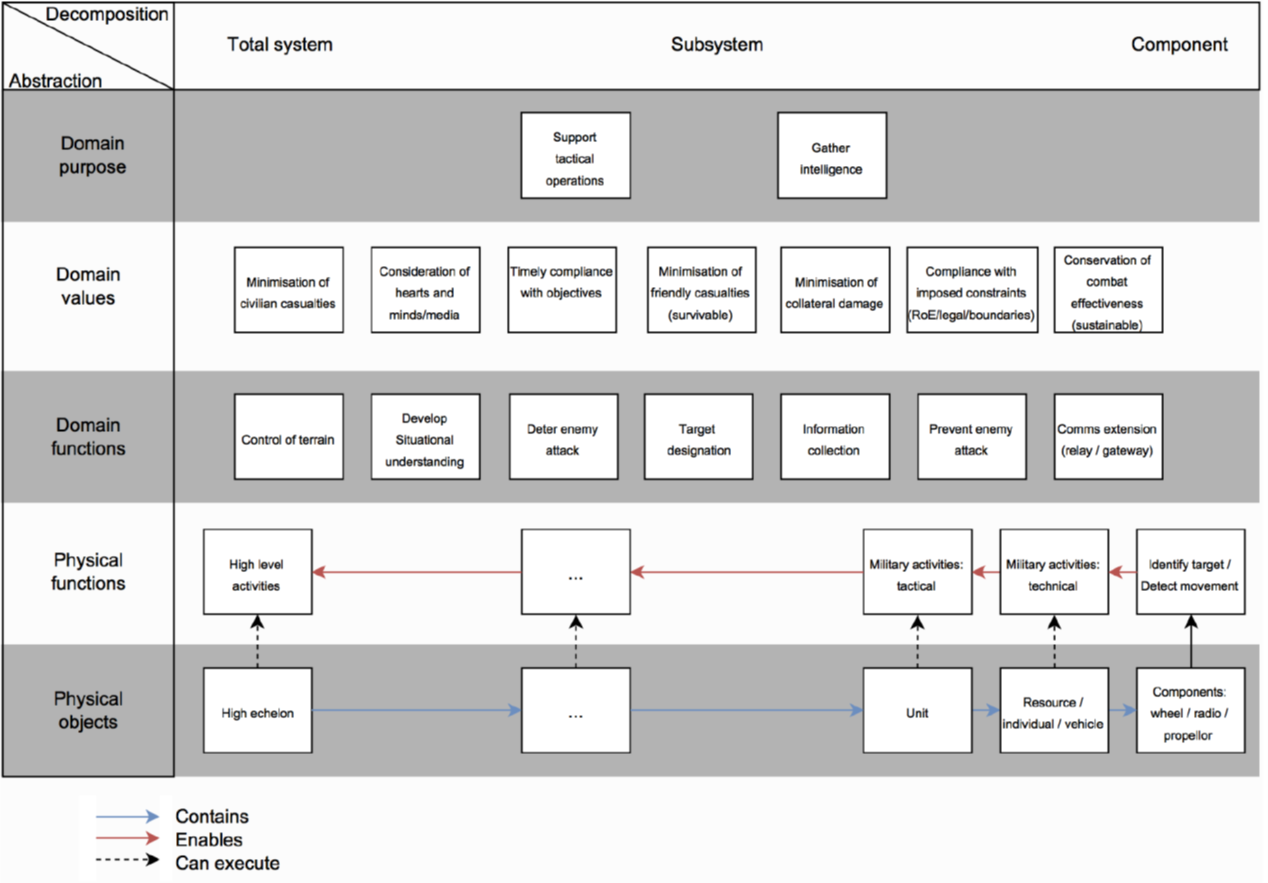
\includegraphics[width=0.4\textwidth]{images/ads.png}
	\caption{The abstraction decomposition space for the UV domain}
	\label{fig:ads}
\end{figure}
%
Playbook describes the physical functions in terms of what tasks have to be executed. However, intelligent autonomous systems have the ability to adjust their behavior and therefore require normative information about how they should execute tasks, e.g. fast, careful or aggressive. Normative guidelines should provide information how physical functions have to be executed and allow intelligent systems to adjust their behavior to the situation and preferences of the user, which are typically described in the commander's intent. We propose to extend the abstraction layer with these normative guidelines. Since the guidelines describe how physical functions should be executed, they will be included at the same level of abstraction in the ADS.
\\\\
While normative guidelines can be integrated in and communicated to systems through a formalized language such as the Battle Management Language (BML) (Carey et al, 2001; Hieb and Schade, 2007), it is not obvious how to represent these terms to make them understandable for a system. According to Hazen and Randall (2008), translating the preferences of a user into settings for parameters seems promising to communicate the commander's intent to systems. Follow up research can investigate the usability of sets of fixed settings for parameters that represent specific terms so they can be communicated by a formal language such as BML. For example, aggressive could be represented by the settings high speed, high risk acceptance and a high amount of vehicles. To use parameters, we need to identify those parameters that can cover the normative guidelines of the user for a specific task.
%
% Argumentation for the choice of parameters
%
The identified user values for a specific process (e.g. the scheduling of tasks to vehicles) are useful to identify the normative requirements of the user about how the physical functions within that process should be executed. It is important that the normative requirements are reflected in the outcome of the situation, otherwise it would decrease the trust of the user in the system (TODO: add alignment of objectives reference). Several of the parameters might have an "optimal" setting when isolated from other user preferences, e.g. the risk of the loss of a vehicle should always be minimized. However, when other preferences are also considered, there typically is no general optimal setting for each parameter, since each parameter conflicts others. This results in dilemmas for the system, since there is no general optimal solution, the optimum depends on the situation, the commander's intent and/or the user. Therefore, parameters that conflict each other and thus require user decisions should be identified during the design phase of a system already so the conflicts can be tackled. The identified normative requirements for the scheduling example are shown below per user value with the possible settings for each parameter. The user values about the physical execution of the tasks are not considered, since that would require more insight in the capabilities of the resources which currently do not exist. We only focused on those user values (see Figure \ref{fig:ads}) important for the scheduling phase. 
%
\begin{itemize}
	\item Effective use of resources
		\begin{itemize}
			\item Information quality and quantity: dependent on information requirements
		\end{itemize}
	\item Efficient use of resources
		\begin{itemize}
			\item Time pressure: Very low (1) - Very high (5)
			\item Fuel consumption: Keep low (1) - Not restricted (5)
		\end{itemize}
	\item Compliance with imposed constraints
		\begin{itemize}
			\item Secrecy: Overt (a) / Covert (b)
		\end{itemize}
	\item Safety
		\begin{itemize}
			\item Risk acceptance: Take no risk (1) - Take risk (5)
		\end{itemize}
	\item Conservation of combat effectiveness
		\begin{itemize}
			\item Massiveness: Use few resources (1) - Use many resources (5)
		\end{itemize}
\end{itemize}
%
On top of these parameters that represent the normative requirements, there may also be constraints to support user values, for example constraints considering time or location to support deconfliction. These constraints are not further discussed in this paper\footnote{See the full thesis for a description about constraints on the order of tasks and on the allocation of tasks to vehicles}.
\\\\
The full thesis shows an example of a prototype for an interaction design pattern (proto-pattern) to communicate these parameters to the system. 
% Playbook
% Commander's intent
% Physical behavior
% Requires ADS

% //////////// SYSTEM TRANSPARENCY /////////////

\section{System transparency}\label{sec:transparency}
The alignment of the objectives of the user and system should lead to improved user performance. The challenge for the user now is to understand the reasoning of the system behind a certain outcome. In complex situations, this might be impossible, thus the system has to be transparent about its decisions. Considering that parameters are often conflicting, it might be very hard for the user to understand why a certain solution is better than another solution. We investigated possibilities to increase the system's transparency about this matter. 
\\\\
% Insert parameter-dillemas image, but add the fuel consumption parameter
Transparency information should provide insight in the consequences of decisions on which the operator focuses, these are the physical functions (TODO: Find source in literature for this). These consequences reflect on one abstraction level higher in the ADS, the domain functions (military effects). For example, when a reconnaissance task is not executed, the consequence is that the domain function "develop situational understanding" is not fully accomplished. The consequences of breaking normative guidelines also reflect on the domain functions, e.g. when not enough resources were used, the action may not have worked sufficiently to deter the enemy. 
\\\\
The dilemmas between the normative guidelines of the user might lead to user confusion about decisions of the system, this is supported by the results of the user study. A system should provide more transparency about the reasoning behind a certain output. We focus on providing transparency about the dilemmas between the normative guidelines of the user, in order to support the user's understanding that adjustment of the solution would result in worse performance for other guidelines. The amount of guidelines can vary, depending on the phase of the operation. Besides, all guidelines might conflict all the other guidelines and the transparency information should improve the understanding of the dilemma between these parameters. These characteristics require a flexible method to adjust the transparency information to the situation. 
\\\\
A suitable method to make the system more transparent, considering the requirements, is the use of a pie chart icon. These icons can show the compliance of the solution of the system with the user objectives. Each component of the pie chart shows a letter that corresponds with an objective, in this case a normative guideline. The size and color of the component is relative to the performance of the system's solution related to the intent of the user for that normative guidelines, on a scale of 0 (red) to 100 (green). The pie chart-shape makes it more intuitive that expansion of one component of the pie chart (so better compliance with a specific normative guideline) requires other pieces of the pie chart to shrink. This represents the dilemma about the conflicts between the normative guidelines. This method to improve system transparency is already used and proven to be effective in prior research by Mercado et al. (2016), who used a pie chart as a sprocket graphic for a similar case, but with three fixed parameters.  
\\\\
The effects of the use of eSupport are investigated with a user study, this is described in the next paragraph.

\section{Method}

\subsection{Participants}
Participants are a convenience sample of 24 adults and included 16 men and 8 women. All participants were students, former student and employees of the Technical University of Delft. 2 participants had 2 years of military experience. 

\subsection{Apparatus}
The experiment required two monitors, a Dell 24-in. LED color monitor was used to show the missions and required a mouse for interaction. A Philips 17-in. LED color monitor was used to show the instructions and required keyboard for interaction. See Figure 4.1 for an overview. The experiment required the CommonSense Framework of TNO with the additional eSupport application for the scheduling task. The instructions were shown using Microsoft PowerPoint. An Hewlett Packard Spectre 13-3000 notebook was used to run the CommonSense Framework with eSupport applications and a Dell Latitude E6530 notebook to run PowerPoint. An additional A4-paper (cheat-)sheet (see I) provided the participants with basic information, which was also shown during the instruction. The participants were allowed to use this sheet during the missions.

\subsection{Dependent measures}
Dependent measures included operator performance measures (appropriate (non-)compliance, scheduling duration and SA), self assessed trust and CTL (raw NASA-TLX). 

\subsection{Procedure}
After receiving a description of the experiment and giving informed consent, participants filled out a demographic survey and an attentional control questionnaire. Participants then received an instruction about the framework and eSupport for about 30 minutes and consisted of PowerPoint slides concluded with a proficiency test. 
\\\\
At the completion of the training, participants executed 2 mission blocks of 4 missions each. One of two mission blocks provided additional transparency information. The first mission of each block was a training mission and the proposed schedule in the third missions were not optimal. For each mission, the participants received a written partial operations order about the situation, the commander’s intent and the restrictions, which they had to read before starting each mission. Before the first mission they also received a more general description of the military situation and environment. All separate missions take place within this general context. During each mission, the participants had to indicate the commander’s intent to eSupport and insert the given restrictions. These restrictions only consisted of the constraints that a certain UV shall not execute a certain task. Thereafter, the participants had to check if the schedule suggested by eSupport complied to their intent most optimally. They finished each mission by indicating if they would execute the schedule as such, or if they would have liked to adjust it manually. Besides, they gave a rating to each schedule about how optimal they thought it was.

\subsection{Experimental design}
The experiment employs a mixed-factorial design with the transparency condition as independent within-subjects variable and the order of providing the additional transparency as independent between-subjects variable. Each participant executes two mission blocks of four missions each. In one of two mission blocks, additional transparency was provided, the block that provided transparency was counterbalanced.
Besides, to prevent undesired effects of unforeseen differences in the two sets of missions, these were also counterbalanced. The participants were assigned to one of four conditions based on their participant number.
 %------------------------------------------------

\section{Results}
The parameter settings indeed led to user confusion about decisions of the system. 

\begin{table}
\caption{Example table}
\centering
\begin{tabular}{llr}
\toprule
\multicolumn{2}{c}{Name} \\
\cmidrule(r){1-2}
First name & Last Name & Grade \\
\midrule
John & Doe & $7.5$ \\
Richard & Miles & $2$ \\
\bottomrule
\end{tabular}
\end{table}

\blindtext % Dummy text

\begin{equation}
\label{eq:emc}
e = mc^2
\end{equation}

\blindtext % Dummy text

%------------------------------------------------

\section{Discussion}

\subsection{Subsection One}

A statement requiring citation \cite{Figueredo:2009dg}.
\blindtext % Dummy text

\subsection{Subsection Two}

\blindtext % Dummy text

%----------------------------------------------------------------------------------------
%	REFERENCE LIST
%----------------------------------------------------------------------------------------

\begin{thebibliography}{99} % Bibliography - this is intentionally simple in this template

\bibitem[Figueredo and Wolf, 2009]{Figueredo:2009dg}
Figueredo, A.~J. and Wolf, P. S.~A. (2009).
\newblock Assortative pairing and life history strategy - a cross-cultural
  study.
\newblock {\em Human Nature}, 20:317--330.
 
\end{thebibliography}

%----------------------------------------------------------------------------------------

\end{document}
